\documentclass[../thesis.tex]{subfiles}

\begin{document}
\vspace{-1\baselineskip}

\section{The Standard Model}
\label{sec:SM}
The Standard Model of physics (\acs{SM}) is currently the most successful formalism to describe the physical world at a microscopic scale.\\
The \acs{SM} provides descriptions for all currently known elementary particles and three out of four fundamental forces with the exception of gravity.\\
%- limitations: gravity \& general relativity, arbitrary free parameters

\subsection{Elementary particles}
Elementary particles in the \acs{SM} can be classified into two groups: bosons, consisting of particles following Bose-Einstein statistics with integer spin and fermions, consisting of particles following Fermi-Dirac statistics with half-integer spin\\
Fermions are the building blocks of composite particles and consequently all known matter, and can be further split into quarks \& leptons.\\
Bosons act as force mediators for all fundamental forces described by the \acs{SM}. Bosons have two types: a scalar boson with spin $0$ and vector gauge bosons with spin $1$.\\
For each elementary particle there also exists a corresponding antiparticle with identical mass and opposite charge (electric or color).

\begin{figure}[!htbp]
\begin{center}
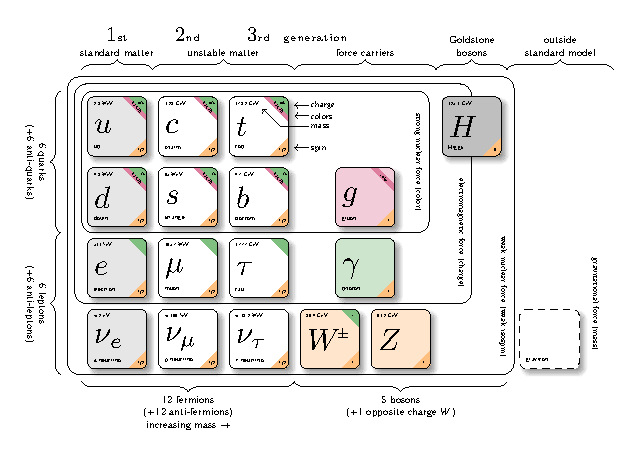
\includegraphics[width=\linewidth]{fig/theory_smparticles.pdf}
\caption{\label{fig:smparticles}\citep{theory:smparticles3}}
\end{center}
\end{figure}

\subsubsection*{Fermions}
Quarks and leptons each has six flavors, grouped into three generations of doublets.\\
The six quark flavors consist of up ($u$), down ($d$), charm ($c$), strange ($s$), bottom ($b$) and top ($t$) quark flavors in increasing order of mass, forming three doublets $(u,d)$, $(c,s)$ and $(t,b)$.\\
Each doublet consists of one quark with electric charge of $+2/3$ ($u$, $s$, $t$), and one with charge of $-1/3$ ($d$, $c$, $b$).\\
Each quark also has a property known as color charge, with possible values of red ($R$), green ($G$), blue ($B$) or antired ($\bar{R}$), antigreen ($\bar{G}$), and antiblue ($\bar{B}$). Color charge follows color confinement rules, which allows only configurations of quarks with neutral color charge to exist in isolation. Neutral charge configurations can be formed from either a set of three colors $(R,G,B)$, a set of a color and its anticolor $(q,\bar{q})$, or any combination of the two. Consequently, no isolated quark can exist in a vacuum and can only exist in bound states called hadrons.\\
Quarks are the only elementary particles in the SM that can interact with all four fundamental forces.\\
The three leptons doublets consist of electron ($e$), muon ($\mu$), tau ($\tau$) and their respective neutrino flavors: electron neutrino ($\nu_e$), muon neutrino ($\nu_\mu$) and tau neutrino ($\nu_\tau$)\\
Charged leptons ($e$, $\mu$, $\tau$) carry an electric charge of $-1$, while their antiparticles carry the opposite charge $+1$ and their corresponding neutrino flavors carrying no charge (charge neutral).\\
Charged leptons interact with all fundamental forces except the strong force, while neutrinos only interact with the weak force and gravity.

\subsubsection*{Bosons}
The \acs{SM} classify bosons into two types: one scalar boson with spin $0$ known as the Higgs ($H$) boson, and vector gauge bosons with spin $1$ known as gluons ($g$), photon ($\gamma$), $W^\pm$ and $Z$ bosons.\\
The gluons and photon are massless, while the $W^\pm$, $Z$ and $H$ are massive.\\
Each vector gauge boson serves as the mediator for a fundamental force described by the SM.\\
Gluons are massless mediator particles for the strong interaction between quarks according to quantum chromodynamics (\acs{QCD}), and carry the color charge in a strong interaction. Each gluon carries a non-neutral color charge out of eight linearly independent color states in the gluon color octet.\\
Photon is the massless and charge-neutral mediator particle for the electromagnetic interaction following quantum electrodynamics (\acs{QED}).\\
The $W^\pm$ and $Z$ bosons are massive mediator particles for the weak interaction, with the $W^\pm$ boson carrying an electric charge of $\pm 1$ while the $Z$ boson is charge neutral.\\
Other than the vector gauge boson, the only scalar boson in the SM is the Higgs boson which is massive with electric charge of $0$.\\
The Higgs boson does not mediate a fundamental force like vector bosons, but serve to provide the rest mass for all massive elementary particles in the SM through the Higgs mechanism.

\subsection{Mathematical formalism}
The \acs{SM} can be described within the formalism of quantum field theory (\acs{QFT}) with a composite Lagrangian
\begin{equation}
\mathcal{L}_\mathrm{SM} = \mathcal{L}_\mathrm{QCD} + {\underbrace{(\mathcal{L}_\mathrm{gauge}+\mathcal{L}_\mathrm{fermion}+\mathcal{L}_\mathrm{Higgs}+\mathcal{L}_\mathrm{Yukawa})}_{\mathcal{L}_\mathrm{EW}}}
\end{equation}
where $\mathcal{L}_\mathrm{QCD}$ is the \acs{QCD} term and $\mathcal{L}_\mathrm{EW}$ is the electroweak (\acs{EW}) term of the Lagrangian.\\
%QFT treats particles as excitations of their corresponding quantum fields: fermion field $\psi$, electroweak boson fields $W_{1,2,3}$ \& $B$, gluon field $G_\alpha$ and Higgs field $\phi$.\\
The \acs{SM} Lagrangian is gauge invariant under global Poincar\'e symmetry and local $SU(3)_C \times SU(2)_L \times U(1)_Y$ gauge symmetry, with the gauge term $SU(3)_C$ corresponding to the strong interaction and $SU(2)_L \times U(1)_Y$ to the \acs{EW} interaction.\\
Global Poincar\'e symmetry ensures that $\mathcal{L}_\mathrm{SM}$ satisfies translational symmetry, rotational symmetry and Lorentz boost frame invariance. By Noether's theorem, these symmetries give rise to conservation of momentum, angular momentum and energy.

\subsubsection*{Quantum chromodynamics}
\acs{QCD} is a non-Abelian gauge theory (Yang-Mills theory) describing the strong interaction between quarks in the \acs{SM} with the gauge group $SU(3)_C$, where $C$ represents conservation of color charge under $SU(3)_C$ symmetry.\\
According to QFT, quarks can be treated as excitations of corresponding quark fields $\psi$.
Quark fields are invariant under $SU(3)_C$ transformation
\begin{equation}
\psi \rightarrow e^{i\theta(x)T_a} \psi
\end{equation}
where $T_a$ are generators of $SU(3)_C$, represented as $T_a=\lambda_a/2$ with $\lambda_a$ being the eight Gell-Mann matrices.\\
The free Dirac Lagrangian
\begin{equation}
\mathcal{L}_0=\bar{\psi}(i\gamma^\mu\partial_\mu-m)\psi
\end{equation}
is invariant under global $SU(3)$ symmetry, but not under local $SU(3)_C$ symmetry.
To establish invariance under local $SU(3)_C$ symmetry, the gauge covariant derivative $D_\mu$ is defined so that
\begin{equation}
D_\mu \psi = (\partial_\mu-ig_sG^a_\mu T_a)\psi,
\end{equation}
where $g_s=\sqrt{4\pi\alpha_s}$ is the \acs{QCD} coupling constant, $G^a_\mu(x)$ are the eight gluon fields that transform under $SU(3)_C$ as
\begin{equation}
G_\mu^a \rightarrow e^{iT_a\theta_a(x)}\left( G_\mu^a+\frac{i}{g_s}\partial_\mu \right)e^{-iT_a\theta_a(x)}
=G_\mu^a - \frac{1}{g_s}\partial_\mu\theta_a(x)-f_{abc}\theta_b(x)G_\mu^c,
\end{equation} 
and $T_a$ are the generators of $SU(3)_C$ defined as $T_a=\lambda_a/2$ with $\lambda_a$ being the eight Gell-Mann matrices.\\
Defining the gluon field strength tensor $G^a_{\mu \nu}$ as
\begin{equation}
G_{\mu \nu}^a \equiv \partial_\mu G^a_\nu - \partial_\nu G^a_\mu - g_s f^{abc} G^b_\mu G^c_\nu,
\end{equation}
where $f^{abc}$ are the structure constants of $SU(3)_C$, the gauge invariant \acs{QCD} Lagrangian is
\begin{equation}
\mathcal{L}_\text{QCD}=\bar{\psi}(i\gamma^\mu D_\mu-m)\psi - \frac{1}{4} G_{\mu \nu}^a G_a^{\mu \nu},
\end{equation}
which can be expressed in the form of
\begin{equation}
\mathcal{L}_\mathrm{QCD} = 
\underbrace{
-\frac{1}{4} G_{\mu \nu}^a G_a^{\mu \nu}
}_{\substack{\text{gluon kinematics}\\ \text{\& self-interaction}}}
+\underbrace{\vphantom{\frac{1}{4}}
\bar{\psi}\left( i\gamma^\mu \partial\mu-m \right)\psi
}_\text{quark kinematics}
+\underbrace{\vphantom{\frac{1}{4}}
\bar{\psi}^i\left( g_s \gamma^\mu (T_a)_{ij} G^a_\mu \right)\bar{\psi}^j
}_\text{quark-gluon interaction}.
\end{equation}
with $i$, $j$ being the color indices with integer values from $1$ to $3$. The noncommutativity of $SU(3)_C$ gives rise to an additional term consisting of only gluon fields and gluon-gluon interactions. Additionally, the Lagrangian also forces gluons to be massless to maintain gauge invariance.\\

\subsubsection*{Electroweak theory}
The electroweak interaction is the unified description of the weak interaction and electromagnetism under the $SU(2)_L \times U(1)_Y$ symmetry group, where $L$ represents the left-handed chirality of the weak interaction and $Y$ represents the weak hypercharge quantum number. The quantum number associated with the weak chirality is the weak isospin $I$. The \acs{EW} quantum numbers are connected by the Gell-Mann-Nishijima relation
\begin{equation}
Q = I_3 + Y/2
\end{equation}
where $Q$ is the electric charge and $I_3$ is the third component of weak isospin $I$.\\
Fermions can have either left-handed or right-handed chirality, and can be divided into left-handed doublets and right-handed singlets
\begin{align}
\psi_L &= \displaystyle\binom{\nu_e}{e_L}, \displaystyle\binom{\nu_\mu}{\mu_L}, \displaystyle\binom{\nu_\tau}{\tau_L}, \displaystyle\binom{u_L}{d_L}, \displaystyle\binom{c_L}{s_L}, \displaystyle\binom{t_L}{b_L} \\
\psi_R &= e_R, \mu_R, \tau_R, u_R, d_R, c_R, s_R, t_R, b_R,
\end{align}
with the exception of neutrino which can only have left-handed chirality in the \acs{SM}.\\
Both left-handed and right-handed fermion fields are invariant under $U(1)_Y$ transformation
\begin{equation}
\psi \rightarrow e^{iY\theta(x)/2} \psi.
\end{equation}
Similar to \acs{QCD}, to establish invariance under local $U(1)_Y$ symmetry, the $U(1)_Y$ gauge covariant derivative $D_\mu$ is defined as
\begin{equation}
D_\mu \phi = \left( \partial_\mu -ig' \frac{Y}{2} B_\mu \right) \psi
\end{equation}
where $B_\mu(x)$ is a vector gauge field that transforms under $U(1)_Y$ as
\begin{equation}
B_\mu \rightarrow B_\mu + \frac{1}{g'}\partial_\mu \theta(x)
\end{equation}
and $g'$ is the $B_\mu$ coupling constant.\\
%The Lagrangian
%\begin{equation}
%\mathcal{L} = \bar{\psi}(i\gamma^\mu D_\mu-m)\psi 
%= \bar{\psi}\left( i\gamma^\mu\partial_\mu-m \right)\psi + \bar{\psi}\left( g\frac{Y}{2}B_\mu \right)\psi
%\end{equation}
%is then invariant under local $U(1)_Y$ symmetry.\\
Right-handed fermion singlets are not affected by $SU(2)_L$ transformation, so fermion fields transform under $SU(2)_L$ as
\begin{align}
\psi_L &\rightarrow e^{iI_3 \vec{\theta}(x)\cdot\vec{\sigma}/2} \psi_L \\
\psi_R &\rightarrow \psi_R.
\end{align}
where $\vec{\sigma}/2$ are generators of $SU(2)_L$ and $\vec{\sigma}$ are Pauli matrices. In order to preserve local symmetry, the gauge covariant derivative for $SU(2)_L$ is defined as
\begin{equation}
D_\mu \psi_L = \left( \partial_\mu - ig\frac{\sigma_i}{2}W_\mu^i \right) \psi_L
\end{equation}
where $W_\mu^i (x)$ ($i=1,2,3$) are three boson gauge fields that transform under $SU(2)_L$ as
\begin{equation}
W_\mu^i \rightarrow e^{i\displaystyle\frac{\sigma_i}{2}\theta_i(x)} \left( W_\mu^i+\frac{i}{g}\partial_\mu \right) e^{-i\displaystyle\frac{\sigma_i}{2}\theta_i(x)}
= W_\mu^i + \frac{2}{g}\partial_\mu \theta_a(x) + \epsilon^{ijk}\theta_j(x) W_\mu^k,
\end{equation}
with $g$ as the gauge coupling constant for $W^i_\mu$, and $\epsilon^{ijk}$ as the structure constant for $SU(2)_L$.\\
The gauge covariant derivative for $SU(2)_L \times U(1)_Y$ can then be written as
\begin{align}
D_\mu \psi_L &= \left( \partial_\mu - ig'\frac{Y_L}{2}B_\mu - ig\frac{\sigma_i}{2}W_\mu^i \right) \psi_L \\
D_\mu \psi_R &= \left( \partial_\mu - ig'\frac{Y_R}{2}B_\mu \right) \psi_R.
\end{align}
Similar to \acs{QCD}, the kinetic term is added by defining field strengths for the four gauge fields
\begin{align}
B_{\mu \nu}   &\equiv \partial_\mu B_\nu - \partial_\nu B_\mu \\
W_{\mu \nu}^i &\equiv \partial_\mu W^i_\nu - \partial_\nu W^i_\mu - g e^{ijk} W^j_\mu W^k_\nu.
\end{align}
The local $SU(2)_L \times U(1)_Y$ invariant \acs{EW} Lagrangian can then be expressed as
\begin{align}
\mathcal{L}_\text{EW} &= i\bar{\psi}(\gamma^\mu D_\mu)\psi - \frac{1}{4}W^i_{\mu\nu}W_i^{\mu\nu} - \frac{1}{4}B_{\mu\nu}B^{\mu\nu} \\
&= \underbrace{\vphantom{\frac{1}{4}}
i\bar{\psi}\left(\gamma^\mu\partial_\mu\right)\psi
}_{\substack{\text{fermion}\vphantom{\frac{1}{4}}\\ \text{kinematics}}}
\underbrace{\vphantom{\frac{1}{4}}
-\bar{\psi}\left(\gamma^\mu g'\frac{Y}{2}B_\mu\right)\psi - \bar{\psi}_L\left(\gamma^\mu g\frac{\sigma_i}{2}W_\mu^i\right)\psi_L
}_\text{fermion-gauge boson interaction}
\underbrace{\vphantom{\frac{1}{4}}
-\frac{1}{4}W^i_{\mu\nu}W_i^{\mu\nu} - \frac{1}{4}B_{\mu\nu}B^{\mu\nu}
}_{\substack{\text{boson kinematics}\vphantom{\frac{1}{4}}\\ \text{\& self-interaction}}}.
\end{align}
The \acs{SM} \acs{EW} bosons can be extracted from $\mathcal{L}_\text{EW}$ by reparameterizing the gauge fields $B_\mu$ and $W_\mu^i$ as
\begin{align}
W^\pm &\equiv \frac{1}{\sqrt{2}}\left(W^1_\mu \mp iW^2_\mu\right) \\ 
\begin{pmatrix}
A \\ Z^0
\end{pmatrix}
&\equiv \begin{pmatrix}
\cos \theta_\text{W} & \sin \theta_\text{W} \\
-\sin \theta_\text{W} & \cos \theta_\text{W}
\end{pmatrix}
\begin{pmatrix}
B_\mu \\ W_\mu^3
\end{pmatrix}
\end{align}
where $\theta_\text{W}\equiv\cos^{-1}\left(g/\sqrt{g^2+g'^2}\right)$ is the weak mixing angle. The \acs{EW} Lagrangian can then be rewritten as
\begin{equation}
\begin{aligned}
\mathcal{L}_\text{EW} =&
\underbrace{\vphantom{\displaystyle\frac{e}{2\sin\theta_\text{W}}}
eA_\mu\bar{\psi}\left(\gamma^\mu Q\right)\psi
}_\text{electromagnetism}
+\underbrace{
\displaystyle\frac{e}{2\sin\theta_\text{W}\cos\theta_\text{W}}\bar{\psi}\gamma^\mu\left(v_f-a_f\gamma_5 \right)\psi Z_\mu
}_\text{neutral current interaction} \\
&+\underbrace{
\displaystyle\frac{g}{2\sqrt{2}}\mathlarger{\sum}_{\psi_L}
\left[ \bar{f}_2\gamma^\mu\left(1-\gamma_5\right)f_1 W_\mu^+ + \bar{f}_1\gamma^\mu\left(1-\gamma_5\right)f_2 W_\mu^- \right]
}_\text{charged current interaction}
\end{aligned}
\end{equation}
where $a_f=I_3$, $v_f=I_3(1-4|Q|\sin^2\theta_\text{W})$ and $f_1$, $f_2$ are up and down type fermions of a left-handed doublet.


\subsubsection*{Higgs mechanism}
fermions \& bosons still massless from previous section, resolved by introduction of the Higgs mechanism\\
(show Higgs field, potential \& Lagrangian)\\
(show minimum of Higgs potential aka VEV)\\
----------------------------------[continue later]----------------------------------



\subsection{Four-top quark production}
\label{sec:4top}
- Top: heaviest particle, strong coupling to many BSM particles in BSM models.\\
- 4top: xsec relevant to and enhanced by many BSM models\\
- Predicted by SM and observed [observation paper]\\
- Predicted xsec and observed xsec\\
- (insert Feynman diagrams)\\
- Decay products \& final state topologies



\section{Beyond the Standard Model}

\subsection*{Top-philic vector resonance}
- (briefly introduce composite pseudo-nambu-Goldstone boson and motivation)\\
- hypothesis: top quark large mass results from high mixing between a "true" top quark and a  colored, fermionic composite state\\
- composite vector resonance can be modeled as a top-philic \Zp boson (without QCD color) or top-philic KK-gluon (with QCD color)\\
- color singlet vector boson (Z') model coupling strongly to top and weakly or not at all to others\\
- (show Lagrangian for interaction)\\
- two body decay \Zp into \ttbar with \mZp in TeV range $\rightarrow$ top mass\\
- decay channels: \ttZp s \& t channels, \tWZp, \tjZp\\
- (show decay width at LO)\\
- (Feynman diagrams here)

\subsection*{Higgs-top Yukawa coupling}
(show Lagrangian of Higgs-top Yukawa coupling)\\
(show dependence of \tttt xsec on Yukawa coupling at LO)
%\subsection*{Effective field theory}
%SMEFT expanding on SM Lagrangian using higher order operators\\
%(show EFT Lagrangian)\\
%quick overview on SMEFT dimension-6 four-fermion operators for BSM interpretation\\
%and Higgs oblique parameter


%\section{Collider physics}
%[pp collision, pdf, cross section, luminosity]
%\subsection*{Luminosity}
%\subsection*{Proton-proton collisions}
%jets, parton shower, hadronization
%\subsection*{Parton distribution function}
%\subsection*{Cross section}


\end{document}